\documentclass[
    article,
    12pt,
    oneside,
    a4paper,
    english,
    brazilian
    ]{abntex2}

% ============================================================
% PACOTES
% ============================================================
\usepackage[utf8]{inputenc}
\usepackage[T1]{fontenc}
\usepackage{lmodern}
\usepackage{geometry}
\usepackage{indentfirst}
\usepackage{setspace}
\usepackage{booktabs}
\usepackage{multirow}
\usepackage{array}
\usepackage{longtable}
\usepackage{graphicx}
\usepackage{epstopdf}
\usepackage[font=small,labelfont=bf]{caption}
\usepackage{subcaption}
\usepackage{float}
\usepackage{tikz}
\usetikzlibrary{arrows.meta, positioning}

% Matemática
\usepackage{amsmath}
\usepackage{amssymb}
\usepackage{siunitx}
\numberwithin{equation}{section}

% Código
\usepackage{listings}
\usepackage{xcolor}
\usepackage{url}

% Citações ABNT
\usepackage[alf]{abntex2cite}
\usepackage{hyperref}
\usepackage{csquotes}

% Ambiente para dicas pedagógicas
\newenvironment{dica}{%
    \par\medskip
    \color{blue!60!black}\small\itshape
}{%
    \par\medskip
}

% ============================================================
% CONFIGURAÇÕES
% ============================================================
\geometry{top=3cm, left=3cm, right=2cm, bottom=2cm}

% Abstract no padrão ABNT (sem recuos, fonte do corpo do texto)
\setlength{\absleftindent}{0cm}
\setlength{\absrightindent}{0cm}
\renewcommand{\abstracttextfont}{\normalfont\normalsize}

\graphicspath{{figuras/}}

% ============================================================
% METADADOS
% ============================================================
\titulo{ENTITY MATCHING EM PRODUTOS DE SUPERMERCADO COM SMALL LANGUAGE MODELS FINE-TUNED}

\autor{Pedro Henrique Medeiros Vieira}

\instituicao{%
    \textbf{Universidade Federal da Paraíba} \\
    Centro de Ciências Sociais Aplicadas \\
    Curso de Ciência de Dados para Negócios
}

\preambulo{Proposta de Trabalho de Conclusão de Curso apresentada ao Curso de Ciência de Dados para Negócios da Universidade Federal da Paraíba, como requisito parcial da disciplina Projeto em Ciência de Dados I, na modalidade Artigo Científico.}

\orientador[Orientador:]{Prof. Hilton Martins de Brito Ramalho}

\local{João Pessoa -- PB}
\data{2026}

\begin{document}

\pretextual
\imprimirfolhaderosto
\newpage

% ============================================================
% RESUMO
% ============================================================
\begin{resumo}
% \begin{dica}
% \noindent\textbf{Dica ao autor — Como escrever o Resumo:}
%
% O resumo é o ``cartão de visitas'' do seu trabalho. Muitos avaliadores decidem a qualidade do trabalho a partir dele. Siga a estrutura \textbf{IMRAD}: (1)~\textbf{Contexto}: Qual é o problema? (1-2 frases); (2)~\textbf{Objetivo}: O que o trabalho faz? (1 frase); (3)~\textbf{Método}: Como foi feito? (1-2 frases); (4)~\textbf{Resultados}: O que foi encontrado? (1-2 frases, \textbf{com números!}); (5)~\textbf{Conclusão}: Qual a contribuição? (1 frase). Tamanho recomendado: 150 a 250 palavras para artigos e TCCs. Escreva o resumo \textbf{por último}, quando todo o trabalho estiver pronto. Escolha 3 a 5 palavras-chave que representem os conceitos centrais, separadas por ponto final, em ordem alfabética ou de relevância.
% \end{dica}
\noindent O monitoramento de preços de produtos de supermercado no Nordeste brasileiro, conduzido pelo projeto ALTA (CNPq), enfrenta um problema central de Entity Matching (EM): o mesmo produto físico é descrito com nomes heterogêneos entre diferentes sistemas de ponto de venda (PDV), dificultando sua comparação e análise. Este trabalho propõe investigar o fine-tuning de um Small Language Model (SLM) --- tendo o LLaMA 3.2 3B como candidato principal --- para a tarefa de Entity Matching de produtos, sob a formulação de Cross-Encoder, comparando seu desempenho a métodos tradicionais de similaridade textual e ao mesmo modelo sem especialização (zero-shot). Dada a inexistência de ground truth anotado, a metodologia propõe a construção de um conjunto de treino por supervisão distante e aumentação de dados e de um conjunto de teste padrão-ouro anotado manualmente, de forma independente, sobre dados reais do projeto ALTA, evitando circularidade na avaliação. O trabalho concentra-se na identificação do mesmo produto entre lojas distintas (matching produto--produto, em nível de SKU) e trata o mapeamento de produtos ao dicionário canônico do projeto como fatia secundária, avaliada separadamente, com um adaptador LoRA por tipo de par. Pretende-se contribuir tanto para a infraestrutura analítica do projeto ALTA quanto para a literatura de Entity Matching de baixo recurso em língua portuguesa, lacuna ainda pouco explorada, com potencial de submissão a conferência científica nacional.
\newline
\noindent \textbf{Palavras-chave:} Entity Matching. Small Language Models. Fine-tuning. Produtos de Supermercado. Processamento de Linguagem Natural.
\end{resumo}

\begin{otherlanguage*}{english}
\begin{resumo}[Abstract]
\noindent Price monitoring of supermarket products in Northeastern Brazil, conducted by the ALTA project (CNPq), faces a central Entity Matching (EM) problem: the same physical product is described with heterogeneous names across different point-of-sale (POS) systems, hindering comparison and analysis. This work proposes investigating the fine-tuning of a Small Language Model (SLM) --- with LLaMA 3.2 3B as the primary candidate --- for the product Entity Matching task, under a Cross-Encoder formulation, comparing its performance to traditional text similarity methods and to the same non-specialized (zero-shot) model. Given the absence of annotated ground truth, the methodology proposes building a training set through distant supervision and data augmentation and an independently, manually annotated gold-standard test set over real ALTA project data, avoiding evaluation circularity. The work focuses on identifying the same product across different stores (product-to-product matching at the SKU level) and treats mapping products to the project's canonical dictionary as a secondary slice, evaluated separately, with one LoRA adapter per pair type. It aims to contribute both to the ALTA project's analytical infrastructure and to the still underexplored literature on low-resource Entity Matching in Portuguese, with potential for submission to a national scientific conference.
\newline
\noindent \textbf{Keywords:} Entity Matching. Small Language Models. Fine-tuning. Supermarket Products. Natural Language Processing.
\end{resumo}
\end{otherlanguage*}
\newpage

% ============================================================
% LISTA DE ABREVIATURAS E SIGLAS
% ============================================================
\begin{siglas}
\symboldef{EM}{Entity Matching}
\symboldef{SLM}{Small Language Model}
\symboldef{LLM}{Large Language Model}
\symboldef{PLM}{Pre-trained Language Model (Modelo de Linguagem Pré-treinado)}
\symboldef{PDV}{Ponto de Venda}
\symboldef{PLN}{Processamento de Linguagem Natural}
\symboldef{LoRA}{Low-Rank Adaptation}
\symboldef{QLoRA}{Quantized Low-Rank Adaptation}
\symboldef{ANN}{Approximate Nearest Neighbor}
\symboldef{MRR}{Mean Reciprocal Rank}
\symboldef{NDCG}{Normalized Discounted Cumulative Gain}
\symboldef{MAP}{Mean Average Precision}
\symboldef{TF-IDF}{Term Frequency -- Inverse Document Frequency}
\symboldef{BM25}{Best Matching 25}
\symboldef{VRAM}{Video Random Access Memory}
\symboldef{GPU}{Graphics Processing Unit}
\symboldef{ABNT}{Associação Brasileira de Normas Técnicas}
\symboldef{CNPq}{Conselho Nacional de Desenvolvimento Científico e Tecnológico}
\symboldef{TCC}{Trabalho de Conclusão de Curso}
\symboldef{WDC}{Web Data Commons}
\end{siglas}

% ============================================================
% 1. INTRODUÇÃO E CONTEXTUALIZAÇÃO
% ============================================================
\textual

\section{Introdução e Contextualização}

% \begin{dica}
% \noindent\textbf{Dica ao autor — Como escrever a Introdução:}
%
% A introdução funciona como um \textbf{funil}: começa ampla (contexto geral do tema) e vai estreitando até o problema específico. Ela deve responder a seis perguntas:
% \begin{enumerate}
%     \item \textbf{Qual é o tema?} — Contextualize em 1-2 parágrafos, situando o leitor.
%     \item \textbf{Por que é importante?} — Apresente a relevância com dados ou referências.
%     \item \textbf{O que ainda não sabemos?} — Identifique a lacuna (\textit{gap}) na literatura.
%     \item \textbf{O que este trabalho faz?} — Formule o objetivo geral de forma clara.
%     \item \textbf{Quais são os objetivos específicos?} — Liste de forma mensurável (verbos de ação).
%     \item \textbf{Como o texto está organizado?} — Descreva brevemente as seções seguintes.
% \end{enumerate}
% \textbf{Erro comum:} Começar com a definição do termo central (``\textit{Machine Learning} é uma subárea da IA que...''). Isso pertence à Fundamentação Teórica, não à Introdução. Aqui, \textbf{contextualize o problema}. Tamanho recomendado: 2-3 páginas (artigo/TCC artigo).
% \end{dica}
%
% \begin{dica}
% \noindent\textbf{Dica ao autor:} Equações numeradas devem ser utilizadas com parcimônia, apenas para conceitos verdadeiramente centrais. Use \texttt{\textbackslash begin\{equation\}} para equações que você referenciará ao longo do texto e \texttt{\textbackslash (\textbackslash)} para fórmulas breves no fluxo do parágrafo.
% \end{dica}

O projeto ALTA, vinculado ao CNPq e voltado ao monitoramento de preços de produtos em supermercados dos estados do Nordeste brasileiro (Paraíba, Ceará e Piauí), coleta dados de preços de forma contínua e automatizada. A base resultante contém registros de produtos provenientes de múltiplos estabelecimentos comerciais, cada um com seu próprio sistema de ponto de venda (PDV) e convenções internas de nomenclatura.

O problema central que motiva este trabalho é o de Entity Matching (EM): o mesmo produto físico aparece descrito com nomes radicalmente distintos entre diferentes supermercados. Para que os dados coletados sejam comparáveis e analiticamente úteis, é necessário identificar quando descrições de lojas diferentes se referem ao mesmo produto e, de forma complementar, mapeá-las a um dicionário canônico de produtos mantido pelos pesquisadores do projeto.

Este problema se desdobra em duas subtarefas complementares. A primeira, matching entre a própria base, consiste em identificar que dois registros internos se referem ao mesmo produto físico. A segunda, matching catálogo--dicionário, consiste em mapear um produto da base coletada à sua entrada correspondente no dicionário canônico, composto por aproximadamente 1.500 entradas estruturadas. Este trabalho trata a primeira como tarefa principal e a segunda como complementar (Seção~\ref{sec:delimitacao-escopo}).

A natureza do problema impõe desafios que tornam abordagens clássicas insuficientes:

\begin{itemize}
    \item Abreviações e truncamentos inconsistentes originados nos sistemas de PDV;
    \item Inversão na ordem dos tokens descritivos;
    \item Representações alternativas de unidades de medida (por exemplo, 1L vs. 1000ML vs. 0,9L);
    \item Variação de granularidade descritiva entre lojas;
    \item Marcas e variantes regionais com baixa representação em corpora genéricos;
    \item Ruído tipográfico introduzido pelos sistemas de digitação dos PDVs.
\end{itemize}

A Tabela~\ref{tab:heterogeneidade} ilustra o mesmo produto descrito de formas diferentes em lojas distintas, a partir de dados reais.

\begin{table}[htbp]
\centering
\caption{Exemplos de heterogeneidade nas descrições de produtos}
\label{tab:heterogeneidade}
\small
\resizebox{\textwidth}{!}{%
\begin{tabular}{lll}
\toprule
\textbf{Supermercado A} & \textbf{Supermercado B} & \textbf{Canônico (Dicionário)} \\
\midrule
LEITE INTEGRAL ITALAC 1L & LT ITALAC INTEGRAL 1000ML & Leite Integral Italac 1 Litro \\
OLEO SOJA LIZA 900ML & OLEO COMP SOJA LIZA 0,9L & Óleo Composto de Soja Liza 900ml \\
BISCOITO MARIA BAUDUCCO 200G & BISC M BAUDUCCO 200GR & Biscoito Maria Bauducco 200g \\
\bottomrule
\end{tabular}%
}
\vspace{2mm}
\fonte{Elaborado pelo autor a partir de dados do projeto ALTA}
\end{table}


Este trabalho parte da hipótese de que os métodos tradicionais de comparação de strings --- TF-IDF, BM25, Levenshtein, Jaccard --- e os embeddings semânticos genéricos, sem especialização de domínio, são insuficientes para este problema, em razão da intensidade e da especificidade do ruído presente. A caracterização da base (Seção~\ref{sec:caracterizacao-base}) traz evidência descritiva nessa direção: apenas 2,1\% das descrições se repetem de forma idêntica entre lojas, 60\% dos tipos de token ocorrem em uma única rede, 376 grupos de produtos aparecem com os mesmos tokens em ordens diferentes entre redes e 92\% dos tipos de token da base não ocorrem no vocabulário do dicionário canônico. A blocagem lexical contra o dicionário reforça esse quadro: numa amostra cega de produtos, parte dos que têm entrada correspondente não a tem entre os 100 candidatos mais similares, por abreviação ou por marca que embute a categoria (Seção~\ref{sec:blocagem} e Tabela~\ref{tab:recall-blocagem}). Essa evidência sustenta, mas não demonstra, a hipótese: a comparação de desempenho cabe aos baselines da Seção~\ref{sec:baselines-avaliacao}, mantidos como comparação obrigatória.

\subsection{Delimitação do escopo}
\label{sec:delimitacao-escopo}

Este trabalho concentra-se na subtarefa de matching produto--produto: decidir se duas descrições de lojas distintas correspondem ao mesmo produto, em nível de SKU --- mesma composição, marca, variante e tamanho. É nessa subtarefa que o ruído de PDV pesa mais e da qual depende diretamente a comparação de preços entre lojas. O mapeamento de produtos ao dicionário canônico é tratado como fatia secundária: cada entrada canônica representa um produto genérico, sem marca nem tamanho, e esse matching decide apenas categoria e variante.

Por isso, as duas subtarefas seguem regras de match diferentes e não são intercambiáveis: dois produtos mapeados à mesma entrada canônica pertencem à mesma categoria, mas não são necessariamente o mesmo produto --- o mesmo arroz em embalagens de 1 kg e de 5 kg, por exemplo. A transitividade pelo dicionário vale, portanto, apenas para categoria. Embora a formulação de Cross-Encoder (Seção~\ref{sec:formulacao-modelo}) classifique pares independentemente de sua origem, cada tipo de par recebe um adaptador LoRA próprio sobre o mesmo modelo-base, treinado e avaliado separadamente, e cada fatia tem seu próprio conjunto de teste, extraído do mesmo esforço de anotação (Seção~\ref{sec:construcao-dataset}). [a definir: tamanho do conjunto de teste de cada fatia.]

% ============================================================
% 2. REVISÃO DE LITERATURA
% ============================================================
\section{Revisão de Literatura}

% \begin{dica}
% \noindent\textbf{Dica ao autor — Como escrever a Fundamentação Teórica:}
%
% Esta seção demonstra que você \textbf{domina} o assunto. Mas dominar não é listar --- é \textbf{sintetizar criticamente}. Organize por \textbf{eixos temáticos} (não por autor). Por exemplo: primeiro defina os conceitos gerais (aprendizado supervisionado), depois os modelos específicos (Regressão Logística, RF, LightGBM), e finalmente as métricas de avaliação.
%
% \textbf{O que NÃO fazer} (colagem de citações): ``Segundo Silva (2020), X. De acordo com Santos (2021), X. Para Oliveira (2022), X.'' ← Isso é um catálogo.
%
% \textbf{O que FAZER} (síntese): ``A definição de X evoluiu. Enquanto Silva (2020) enfatiza A, Santos (2021) amplia ao incluir B. Oliveira (2022) propõe uma integração de ambos, argumentando que C.'' ← Aqui você compara, conecta e avalia.
%
% Inclua uma subseção de \textbf{Trabalhos Correlatos}: o que já foi feito de similar? Quais resultados obtiveram? \textbf{Como seu trabalho se diferencia?} Use \texttt{\textbackslash citeonline\{\}} quando o autor é sujeito da frase; \texttt{\textbackslash cite\{\}} para citações indiretas ao final do período.
% \end{dica}

A tarefa de Entity Matching (EM) --- também referida como resolução de entidades ou vinculação de registros --- consiste em decidir se duas descrições referem-se à mesma entidade do mundo real, e constitui etapa central em pipelines de integração de dados. \citeonline{mudgal2018} exploraram sistematicamente o espaço de projeto de arquiteturas de aprendizado profundo para EM, no trabalho que originou o sistema DeepMatcher, demonstrando que abordagens neurais são particularmente eficazes para atributos textuais heterogêneos mal atendidos por funções simples de similaridade de strings --- precisamente o regime de ruído observado em dados de PDV. Ainda assim, esses métodos dependem de grandes volumes de dados rotulados e de representações treinadas do zero para cada conjunto de dados.

A adoção de modelos de linguagem pré-treinados (PLMs) baseados em transformers marcou a transição seguinte. \citeonline{brunner2020} compararam empiricamente arquiteturas transformer e transfer learning na tarefa de EM, mostrando que as arquiteturas transformer superam métodos clássicos de aprendizado profundo por uma margem média de 27,5\%. Esse avanço foi consolidado pelo sistema Ditto: \citeonline{li2020} formularam o EM como classificação de pares de sequências sobre PLMs, com três otimizações --- injeção de conhecimento de domínio, sumarização de sequências longas e aumentação de dados. Os autores reportaram ganhos de até 29\% em F1 sobre o estado da arte anterior, além de atingir resultados equivalentes com metade dos dados rotulados --- resultado diretamente relevante ao cenário de rótulos escassos deste trabalho. No domínio específico de produtos, \citeonline{peeters2021} propuseram o fine-tuning de BERT com objetivo duplo para EM --- que combina a classificação binária de match com uma tarefa auxiliar de identificação da entidade real subjacente a cada registro, favorecendo representações mais discriminativas --- e, posteriormente, \citeonline{peeters2022} propuseram o aprendizado contrastivo supervisionado para product matching, trabalho que fundamenta tecnicamente a via de bi-encoder considerada como extensão futura. Em direção complementar, \citeonline{wang2023sudowoodo} propuseram o Sudowoodo, método de aprendizado contrastivo auto-supervisionado de propósito múltiplo para integração e preparação de dados, reduzindo ainda mais a dependência de pares rotulados ao explorar sinais extraídos dos próprios dados não rotulados.

A abordagem por bi-encoder remonta ao Sentence-BERT: \citeonline{reimers2019} propuseram uma modificação da rede BERT com estruturas siamesas e de tripla para derivar embeddings de sentença semanticamente significativos, comparáveis por similaridade de cosseno, reduzindo o custo de encontrar o par mais similar de 65 horas para cerca de 5 segundos. Essa propriedade de escalabilidade é o que torna a geração de candidatos por busca de vizinhos aproximados (ANN) viável sobre milhares de produtos.

Mais recentemente, modelos de linguagem generativos deslocaram a fronteira. \citeonline{peeters2023} avaliaram o ChatGPT em EM sobre dados de produtos, encontrando desempenho geralmente inferior ao de um RoBERTa com fine-tuning, mas com a vantagem de dispensar treinamento adicional e de generalizar para dados não vistos. A investigação direta do fine-tuning de LLMs generativos para EM foi conduzida por \citeonline{steiner2025}, que analisaram o processo em duas dimensões: a representação dos exemplos de treino --- com adição de explicações geradas por LLM --- e a seleção e geração desses exemplos. Este é o trabalho de referência mais próximo da abordagem aqui proposta, ainda que conduzido sobre benchmarks em inglês e sem o perfil de ruído de sistemas de PDV. Como recurso de avaliação, \citeonline{peeters2024wdc} introduziram o WDC Products, um benchmark multidimensional de product matching.

Dois eixos delimitam a lacuna que este trabalho ocupa. O primeiro é o de baixo recurso: \citeonline{kasai2019} observam que, embora métodos de aprendizado profundo atinjam desempenho estado da arte sobre dados de benchmark, eles requerem grandes volumes de dados rotulados, tipicamente indisponíveis em aplicações reais de resolução de entidades, e propõem combinar transfer learning e active learning para mitigar essa dependência. A ausência total de ground truth anotado no projeto ALTA situa este trabalho exatamente nesse regime --- mais severo, inclusive, por partir de zero rótulos. Em direção complementar, \citeonline{tu2022} propuseram um método de adaptação de domínio para resolução de entidades profunda, investigando se um modelo treinado sobre um domínio de origem bem rotulado pode ser adaptado a um domínio-alvo com poucos ou nenhum rótulo --- cenário estruturalmente próximo ao deste trabalho, em que o domínio de produtos de supermercado em português carece de rótulos nativos. Ferramentas clássicas de gerência de EM, como o Magellan \cite{konda2016}, consolidaram o pipeline canônico de blocagem seguida de matching que ainda estrutura o campo e informa a etapa de geração de candidatos aqui adotada.

O segundo eixo é linguístico e de domínio. A literatura de EM concentra-se predominantemente em dados em inglês, com benchmarks consolidados (WDC Products, Amazon-Google, DBLP-ACM). Para o português brasileiro, o trabalho mais próximo identificado trata de tarefa correlata, porém distinta: \citeonline{silva2021} aplicaram Named Entity Recognition a títulos de produtos do maior e-commerce de varejo brasileiro, concluindo que um pipeline clássico de aprendizado de máquina ainda se mostra mais útil que grandes modelos pré-treinados quando se consideram throughput e eficiência. Trata-se, contudo, de extração de atributos (NER), e não de matching de entidades (EM), e sobre dados de e-commerce, não de PDV de supermercado. Não foi identificado trabalho de EM de produtos de supermercado em português brasileiro com o perfil de ruído de sistemas de PDV --- lacuna que justifica a contribuição central desta proposta.

% ============================================================
% 3. OBJETIVOS
% ============================================================
\section{Objetivos}

\subsection{Objetivo Geral}

Desenvolver e avaliar um sistema de Entity Matching para produtos de supermercado baseado no fine-tuning supervisionado de um Small Language Model (SLM), investigando se um modelo especializado no domínio supera métodos tradicionais e modelos genéricos na identificação do mesmo produto entre lojas distintas e, de forma complementar, no mapeamento de produtos ao dicionário canônico, em dados reais do projeto ALTA/CNPq.

\subsection{Objetivos Específicos}
\label{sec:objetivos-especificos}

\begin{itemize}
    \item Construir um conjunto de dados rotulado de pares de produtos (match / não-match) a partir dos dados reais do projeto, combinando supervisão distante por correspondência de marca e unidade normalizada, aumentação de dados e um conjunto de teste padrão-ouro anotado manualmente, com uma fatia produto--produto (principal) e uma fatia produto--dicionário (secundária);
    \item Implementar e avaliar um conjunto de baselines clássicos (TF-IDF, BM25, Levenshtein, Jaccard e embeddings genéricos) como referência comparativa;
    \item Medir o recall da blocagem lexical isoladamente, em amostra anotada sem acesso aos candidatos, para quantificar o teto que a blocagem impõe ao modelo;
    \item Investigar um pipeline progressivo que reserve métodos de menor custo computacional para os casos triviais e o modelo especializado para os casos difíceis;
    \item Realizar o fine-tuning de um SLM (tendo LLaMA 3.2 3B como candidato principal), com um adaptador LoRA por tipo de par, para a tarefa de Entity Matching no domínio-alvo, sob a formulação de Cross-Encoder (classificação de pares);
    \item Avaliar o modelo com métricas adequadas ao problema: Precision, Recall e F1 para classificação binária, além de MRR e Recall@K para a tarefa de ranqueamento de candidatos;
    \item Conduzir experimentos de ablação para isolar as contribuições individuais das decisões metodológicas relevantes (por exemplo, aumentação de dados e mineração de negativos difíceis --- pares não-match textualmente muito similares, como mesma categoria de produto com marcas diferentes, mais informativos ao treino do que negativos amostrados aleatoriamente);
    \item Conduzir análise de erro qualitativa, categorizando as falhas por tipo de ruído (abreviação, unidade, marca, categoria);
    \item Produzir um artigo científico submetível a conferência nacional da área (BRACIS, ENIAC ou PROPOR).
\end{itemize}

As arquiteturas Bi-Encoder (embeddings especializados com recuperação por similaridade) e híbrida (recuperação seguida de reranqueamento) são reconhecidas como direções promissoras, porém deliberadamente situadas como trabalho futuro, em razão do escopo temporal do trabalho.

% ============================================================
% 4. METODOLOGIA
% ============================================================
\section{Metodologia}

% \begin{dica}
% \noindent\textbf{Dica ao autor — Como escrever a Metodologia:}
%
% A metodologia é o seu \textbf{protocolo de laboratório}. Um pesquisador independente deve conseguir reproduzir todo o estudo lendo apenas esta seção. Inclua obrigatoriamente:
% \begin{itemize}
%     \item \textbf{Dados:} Fonte, volume, período de coleta, formato, dicionário de variáveis.
%     \item \textbf{Pré-processamento:} Tratamento de \textit{missing values} (qual estratégia e por quê), \textit{outliers}, codificação, normalização.
%     \item \textbf{Divisão treino/teste:} Proporção e método (\textit{holdout}, \textit{K-fold}, \textit{stratified}).
%     \item \textbf{Algoritmos:} Quais, com quais hiperparâmetros, e por que foram escolhidos.
%     \item \textbf{Métricas:} Quais métricas de avaliação e por que são adequadas para o problema.
%     \item \textbf{Reprodutibilidade:} \textit{Seed}, versões de software, link do repositório.
% \end{itemize}
% Use verbos no \textbf{pretérito perfeito} se os experimentos já foram realizados (``foram treinados'', ``utilizou-se''), ou no \textbf{futuro} se for um projeto de pesquisa (``serão treinados'').
% \end{dica}

\subsection{Construção do conjunto de dados e ground truth}
\label{sec:construcao-dataset}

O maior risco técnico do projeto é a inexistência de ground truth anotado --- condição que inviabiliza treinamento supervisionado e avaliação rigorosa sem trabalho prévio de rotulagem. Este desafio é tratado como parte integrante da contribuição do trabalho, e não como limitação a ser minimizada. A estratégia adotada separa deliberadamente as origens dos rótulos de treino e de teste, de modo a preservar a validade da avaliação.

\textbf{Treino.} O conjunto de treino é construído a partir de mecanismos combinados: (i) supervisão distante --- técnica que deriva rótulos automaticamente de uma fonte estruturada preexistente, sem anotação humana direta ---, em que a correspondência de marca e de unidade normalizada entre dois produtos fornece rótulos provisórios para a fatia produto--produto; (ii) para essa mesma fatia, pares derivados de variantes de títulos de produtos de um projeto da liga acadêmica TAIL/UFPB, particionados por grupo de título original [a confirmar: autorização escrita da TAIL e forma de citação]; (iii) aumentação sintética por perturbação controlada de tokens (abreviação, troca de unidades, inversão de ordem); e (iv) para a fatia produto--dicionário, cuja fonte de pares de treino ainda não está definida, eventualmente a geração de pares assistida por ferramenta da Dharma-AI [a definir: uso da ferramenta de geração, em reavaliação]. Como o dicionário canônico não traz marca nem tamanho, a supervisão distante por marca e unidade não se aplica à fatia produto--dicionário. Ferramentas de geração movidas por modelos de linguagem de grande porte têm uso restrito ao conjunto de treino.

\textbf{Teste e validação.} O conjunto de teste é um padrão-ouro anotado manualmente pelo autor diretamente sobre os dados reais do projeto, de forma independente de qualquer ferramenta de geração, e composto por duas fatias: pares produto--produto (principal) e pares produto--dicionário (secundária) [a definir: tamanho de cada fatia]. Esta separação é uma decisão metodológica central: caso o conjunto de teste fosse produzido por uma ferramenta baseada em modelo de linguagem, a avaliação seria circular e mediria a aderência do modelo à distribuição do gerador, e não sua capacidade de resolver o problema real. Por isso, nenhum gerador ou modelo de linguagem produz ou rotula pares de teste ou de validação. Os produtos que compõem o conjunto de teste são removidos da base que alimenta o treino, aplicando-se a partição antes de qualquer geração ou aumentação, de modo a impedir vazamento.

\textbf{Confiabilidade da anotação.} Sendo a anotação conduzida por um único anotador, não é aplicável o cálculo de concordância inter-anotadores (Cohen's Kappa). Adota-se, em seu lugar, um procedimento de teste-reteste (concordância intra-anotador): um subconjunto correspondente a pelo menos 50\% do conjunto de teste é reanotado após intervalo de pelo menos sete dias, sem acesso aos rótulos originais, e a concordância entre as duas passagens é reportada como medida de consistência interna (faixa desejável de Kappa superior a 0,75), calculada separadamente para cada tipo de par, já que as regras diferem. Casos genuinamente indecidíveis recebem rótulo transitório e são adjudicados por consulta ao dicionário canônico oficial, não integrando o conjunto de teste. A alternativa de recrutar um segundo anotador --- ainda que sobre um subconjunto restrito e sem acesso ao pipeline de geração e às heurísticas de supervisão distante, o que permitiria reportar uma concordância inter-anotadores genuína --- foi considerada e descartada por indisponibilidade de um colaborador com esse perfil no horizonte deste trabalho; o risco de vazamento de critério do treino para os rótulos de teste, decorrente de o mesmo autor conhecer ambas as etapas, é reconhecido explicitamente como limitação, mitigada apenas parcialmente pelo teste-reteste.

\textbf{Guidelines de anotação.} As regras de decisão para match/não-match diferem por tipo de par e estão documentadas em protocolo próprio (\texttt{docs/protocolo\_anotacao.md}, repositório do projeto), mantido como artefato versionado e auditável. Em pares produto--produto, decidem composição, marca, variante e tamanho (1 kg e 5 kg são produtos distintos). Em pares produto--dicionário, cuja entrada canônica é um produto genérico sem marca nem tamanho (por exemplo, uma única entrada ``ARROZ BRANCO'', sem variantes por marca ou tamanho de embalagem, como confirma o dicionário recebido do projeto ALTA), decidem apenas categoria e variante; kit ou promoção e marca própria declarada na descrição são não-match.

\textbf{Divisão dos dados e prevenção de vazamento.} Na fatia produto--dicionário, o particionamento é estratificado por produto canônico: todos os pares que envolvem um dado produto do dicionário permanecem integralmente em uma única partição, com proporção sugerida de 70\% para treino, 15\% para validação e 15\% para teste. Na fatia produto--produto, nenhum produto aparece em mais de uma partição [a definir: unidade de partição dessa fatia]. A aumentação sintética é aplicada exclusivamente ao treino, após o particionamento. O dicionário canônico recebido possui uma coluna adicional (\texttt{cod\_padrao}) cujo significado não foi confirmado com o time do ALTA e que concentra 82,7\% das 1.593 entradas em um único valor (99); por essas duas razões, optou-se por não utilizá-la como sinal de categoria, de modo que a estratificação e a geração de candidatos não incorporam balanceamento por categoria de produto.

\subsection{Formulação e modelo}
\label{sec:formulacao-modelo}

O problema é formulado como uma tarefa de Cross-Encoder: dado um par de descrições de produtos, o modelo produz uma decisão binária de match / não-match. Esta formulação privilegia a precisão e simplifica a avaliação; seu custo de inferência quadrático é mitigado por uma etapa prévia de blocagem, feita sobre o dicionário canônico (cerca de 1.500 entradas) na fatia secundária e sobre os produtos das demais lojas na fatia principal (Seção~\ref{sec:blocagem}). Cada tipo de par recebe um adaptador LoRA próprio sobre o mesmo modelo-base.

A seleção do SLM segue critérios explícitos de tamanho, suporte a português, custo de fine-tuning e licença, resumidos na Tabela~\ref{tab:criterios_slm}. A comparação é deliberadamente restrita a modelos na faixa de 2 a 4 bilhões de parâmetros, e não estendida a modelos maiores (10 a 30 bilhões de parâmetros, quantizados e/ou com arquitetura de mistura de especialistas) que a infraestrutura de treino da Dharma-AI também suportaria em inferência: o critério decisivo é a viabilidade de operação continuada do modelo fine-tuned pelo próprio projeto ALTA após o encerramento deste trabalho, sem depender de GPUs de alta capacidade (48 a 141 GB de VRAM) cuja disponibilidade de longo prazo para a infraestrutura de produção do ALTA não está garantida. Um modelo na faixa de 2 a 4 bilhões de parâmetros preserva essa portabilidade operacional mesmo em hardware modesto. Adota-se o LLaMA 3.2 3B como candidato principal, por ser o único dos três a listar explicitamente o português entre seus idiomas de suporte, por equilibrar custo de adaptação e capacidade, e por dispor de documentação madura --- fatores relevantes ao horizonte temporal do trabalho. O Gemma 2 2B é mantido como candidato secundário de menor custo.

\begin{table}[htbp]
\centering
\caption{Critérios de seleção do SLM}
\label{tab:criterios_slm}
\small
\resizebox{\textwidth}{!}{%
\begin{tabular}{lccc}
\toprule
\textbf{Critério} & \textbf{LLaMA 3.2 3B} & \textbf{Gemma 2 2B} & \textbf{Phi-3 Mini (\textasciitilde{}3,8B)} \\
\midrule
Licença & Llama Community License & Gemma Terms of Use & MIT \\
Parâmetros / custo & 3B / intermediário & 2B / menor custo & 3,8B / maior \\
Suporte a português & Explícito (8 idiomas) & Multilíngue amplo & Multilíngue, sem foco declarado \\
Documentação & Madura & Boa & Boa \\
\bottomrule
\end{tabular}%
}
\vspace{2mm}
\fonte{Elaborado pelo autor a partir da documentação oficial dos modelos}
\end{table}


% \begin{dica}
% \noindent\textbf{Dica ao autor:} As tabelas geradas pelos scripts Python são salvas em \texttt{latex/tabelas/} e importadas com \texttt{\textbackslash input\{../tabelas/nome\}}. Isso garante que, ao reexecutar o pipeline, os dados da tabela sejam atualizados sem que você precise editá-los manualmente.
% \end{dica}
%
% \begin{dica}
% \noindent\textbf{Dica ao autor:} Sempre referencie as figuras no texto antes de apresentá-las. Use \texttt{\textbackslash label\allowbreak \{fig:nome\}} e \texttt{\textbackslash ref\{fig:nome\}} para referência cruzada. O prefixo \texttt{fig:} ajuda a organizar as labels. Para figuras geradas pela pipeline, os arquivos \texttt{.eps} estão em \texttt{latex/figuras/}.
% \end{dica}

O fine-tuning será conduzido por meio de LoRA (Low-Rank Adaptation) em precisão bf16, sem quantização de 4 bits. LoRA insere matrizes treináveis de baixo posto em camadas do modelo, mantendo os pesos originais congelados --- reduzindo drasticamente o número de parâmetros ajustados; bf16 é um formato de ponto flutuante de 16 bits com a mesma faixa dinâmica do float32, evitando os problemas de overflow numérico comuns em fp16. Essa escolha é viabilizada pela infraestrutura da Dharma-AI, que disponibiliza GPUs com 48 GB (NVIDIA L40S) a 141 GB (NVIDIA H200) de memória de vídeo --- capacidade ampla para um modelo de 3 bilhões de parâmetros, tornando a quantização agressiva desnecessária e preservando maior precisão numérica no ajuste fino. [a confirmar oficialmente com o time de plataforma da Dharma-AI: configuração de produção vs. configuração de testes do ambiente.]

\textbf{Plano de contingência computacional.} Caso a infraestrutura da Dharma-AI se torne indisponível, atrase ou ofereça VRAM inferior ao documentado, duas mitigações estão previstas: (i) migração para recursos de nuvem acadêmica ou Google Colab Pro como ambiente alternativo de treino; e (ii) redução do modelo-alvo para o Gemma 2 2B, candidato secundário já justificado na Tabela~\ref{tab:criterios_slm}, que demanda menos memória e mantém o cronograma viável sem necessidade de requalificar o pipeline de fine-tuning.

\subsection{Blocagem e formulação de recuperação}
\label{sec:blocagem}

A Figura~\ref{fig:pipeline} sintetiza o encadeamento entre blocagem lexical, geração de candidatos, reranqueamento pelo Cross-Encoder, roteamento pelo pipeline progressivo e a comparação experimental contra os baselines, descrito em detalhe ao longo desta e das próximas subseções.

\begin{figure}[htbp]
\centering
\caption{Pipeline de blocagem, matching e avaliação comparativa}
\label{fig:pipeline}
\begin{tikzpicture}[
    node distance=0.8cm and 1.4cm,
    box/.style={draw, rectangle, rounded corners, align=center, minimum height=1cm, text width=4.8cm, font=\small},
    decision/.style={draw, rectangle, rounded corners, align=center, minimum height=1.1cm, text width=5.6cm, font=\small},
    wide/.style={draw, rectangle, rounded corners, align=center, minimum height=1.2cm, text width=10.5cm, font=\small},
    arrow/.style={-Latex}
]

\node[box] (input) {Produto de entrada\\(descrição PDV)};
\node[box, below=of input] (blocagem) {Blocagem lexical\\(TF-IDF / BM25)};
\node[box, right=1.8cm of blocagem] (dicionario) {Dicionário canônico\\(\textasciitilde{}1.500 entradas)};
\node[decision, below=1.3cm of blocagem] (progressivo) {Pipeline progressivo: score do baseline lexical acima do limiar de confiança?};
\node[box, below left=1.6cm and -0.9cm of progressivo] (aceita) {Aceita decisão do baseline lexical (barato, sem SLM)};
\node[box, below right=1.6cm and -0.9cm of progressivo] (crossencoder) {Cross-Encoder fine-tuned (reranqueamento + decisão match / não-match)};
\node[box, below=3.6cm of progressivo] (decisao) {Decisão final: match / não-match};
\node[wide, below=1.3cm of decisao] (comparacao) {Comparação experimental (Seção~\ref{sec:baselines-avaliacao}) --- mesmo conjunto de teste:\\TF-IDF, BM25, Levenshtein, Jaccard, embeddings genéricos, LLaMA 3.2 3B zero-shot\\$\rightarrow$ Precision, Recall, F1, MRR, Recall@K, teste de McNemar};

\draw[arrow] (input.south) -- (blocagem.north);
\draw[arrow] (dicionario.west) -- (blocagem.east);
\draw[arrow] (blocagem.south) -- node[right, font=\tiny] {top-$k$ candidatos} (progressivo.north);
\draw (progressivo.south) -- ++(0,-0.4) coordinate (fork);
\draw[arrow] (fork) -| node[pos=0.12, above, font=\tiny] {sim} (aceita.north);
\draw[arrow] (fork) -| node[pos=0.12, above, font=\tiny] {não} (crossencoder.north);
\draw[arrow] (aceita.south) |- (decisao.west);
\draw[arrow] (crossencoder.south) |- (decisao.east);
\draw[arrow] (decisao.south) -- (comparacao.north);

\end{tikzpicture}
\vspace{2mm}
\fonte{Elaborado pelo autor}
\end{figure}


A blocagem --- etapa que reduz o espaço de candidatos antes da aplicação do Cross-Encoder --- é realizada por meio de TF-IDF ou BM25 --- sobre o dicionário canônico, na fatia produto--dicionário, e sobre os produtos de lojas distintas, na fatia produto--produto ---, reaproveitando os mesmos métodos já implementados como baselines (Seção~\ref{sec:baselines-avaliacao}). Para cada produto de entrada, os k candidatos mais similares do dicionário (ou dos produtos das demais lojas) são recuperados por similaridade lexical, e o Cross-Encoder pontua cada par (produto, candidato) com uma probabilidade de match. É importante demarcar que essa blocagem é um filtro lexical clássico, não uma arquitetura Bi-Encoder aprendida: a decisão de matching permanece inteiramente a cargo do Cross-Encoder, e o termo ``formulação de Cross-Encoder'' refere-se a esse modelo de decisão, não ao pipeline de produção como um todo --- distinção também adotada por trabalhos que tratam a blocagem como etapa independente do modelo de matching \cite{thirumuruganathan2021}.

Essa arquitetura de recuperação define precisamente as métricas de ranqueamento: o Recall@K mede se o match verdadeiro está entre os k candidatos retornados pela blocagem após o reranqueamento do Cross-Encoder, e o MRR é calculado sobre a posição do match verdadeiro nessa lista reordenada. Consequentemente, a blocagem impõe um teto de recall que o Cross-Encoder não recupera sozinho --- limitação que será quantificada reportando-se o recall da blocagem isoladamente, antes do reranqueamento.

Na fatia produto--dicionário, o recall da blocagem isolada foi medido numa amostra cega de 50 produtos distintos, sorteados com seed fixa, em que o autor indicou a entrada correta do dicionário sem ver os candidatos --- medir o recall apenas sobre os pares anotados do teste seria otimista, pois os casos que a blocagem perde nunca seriam anotados. A Tabela~\ref{tab:recall-blocagem} mostra que o TF-IDF iguala ou supera o BM25 em todos os valores de k e que o recall se estabiliza a partir de 50 candidatos, num teto imposto por produtos sem nenhuma palavra em comum com a entrada correspondente, como abreviações (\texttt{CERV}) e marcas que embutem a categoria (\texttt{NESCAFE}). Os produtos sem entrada adequada no dicionário ficam fora do cálculo e são contados à parte. Adotou-se o TF-IDF com $k=20$, congelado antes da construção do conjunto de teste. Na fatia produto--produto, a blocagem é feita entre produtos de lojas distintas, sob o mesmo princípio lexical, e a medição do seu recall é etapa em execução.

% Gerado automaticamente por scripts/03_construcao_dataset.py — não editar à mão.
\begin{table}[htbp]
\centering
\caption{Recall da blocagem isolada, por método e número de candidatos (k), na amostra cega}
\label{tab:recall-blocagem}
\small
\begin{tabular}{lcc}
\toprule
\textbf{k} & \textbf{TF-IDF} & \textbf{BM25} \\
\midrule
1 & 45,2\% & 42,9\% \\
5 & 81,0\% & 73,8\% \\
10 & 83,3\% & 81,0\% \\
20 & 85,7\% & 83,3\% \\
50 & 90,5\% & 90,5\% \\
100 & 90,5\% & 90,5\% \\
\bottomrule
\end{tabular}
\vspace{2mm}
\fonte{Elaborado pelo autor (amostra cega: 42 produtos com entrada correspondente; 8 sem entrada e 0 incertos, fora do cálculo)}
\end{table}


\subsection{Baselines e avaliação}
\label{sec:baselines-avaliacao}

Antes de qualquer modelo especializado, um conjunto de baselines clássicos (TF-IDF, BM25, Levenshtein, Jaccard e embeddings genéricos) será implementado e avaliado sobre o mesmo conjunto de teste de cada fatia, com protocolo de avaliação congelado. Adicionalmente, o próprio LLaMA 3.2 3B sem fine-tuning (zero-shot, via prompt estruturado para a decisão de match/não-match) compõe o conjunto de baselines. O uso do mesmo modelo-base do fine-tuning como baseline zero-shot isola o efeito da especialização: eventuais diferenças de desempenho são atribuíveis ao processo de fine-tuning, e não a diferenças de arquitetura ou capacidade do modelo --- condição necessária para testar integralmente a hipótese central deste trabalho, que contrapõe o modelo especializado tanto a métodos tradicionais quanto a modelos genéricos.

A avaliação reportará Precision, Recall e F1 para a decisão binária e, para o ranqueamento de candidatos, MRR e Recall@K. A diferença de desempenho entre o modelo especializado e os baselines será submetida a teste de significância estatística, em resposta direta à hipótese central (Seção~\ref{sec:hipotese-central}). As duas fatias são avaliadas e reportadas separadamente, cada uma com seu adaptador e sua regra de match (Seção~\ref{sec:delimitacao-escopo}): a fatia produto--produto responde à hipótese central e a fatia produto--dicionário, à hipótese secundária (Seção~\ref{sec:hipotese-central}).

Na fatia produto--dicionário, o mapeamento atualmente produzido pelo projeto ALTA é avaliado como baseline adicional; suas predições são consultadas apenas após o congelamento do conjunto de teste e nunca são usadas como rótulo, treino ou validação.

Como comparação externa exploratória, restrita à fatia produto--produto, o modelo é avaliado num benchmark de pares de anúncios de marketplace construído pela liga acadêmica TAIL/UFPB, reportado em tabela separada e rotulado como exploratório: o número reduzido de pares positivos (30) limita o poder estatístico, e o limiar de decisão do modelo é definido na validação deste trabalho, nunca no benchmark. [a confirmar: autorização escrita da TAIL e forma de citação.]

\subsection{Pipeline progressivo}

A investigação do pipeline progressivo (Seção~\ref{sec:objetivos-especificos}) é operacionalizada como uma análise pós-hoc sobre as saídas já geradas na Seção~\ref{sec:baselines-avaliacao}: define-se um limiar de confiança sobre a pontuação do baseline lexical mais forte (TF-IDF ou BM25) acima do qual a decisão de match/não-match é aceita sem consultar o SLM. Pares abaixo desse limiar --- os casos ambíguos --- são roteados ao Cross-Encoder fine-tuned. A análise mede a fração de pares resolvida pelo método barato, a economia computacional resultante e a eventual perda de acurácia frente a rodar o SLM sobre a totalidade dos pares, reaproveitando as avaliações da Semana 12 sem exigir novo treinamento.

\subsection{Reprodutibilidade}

A reprodutibilidade é tratada como requisito. O código será disponibilizado em repositório público após a defesa, com seeds fixas em todas as etapas estocásticas (particionamento, geração e treino), configurações versionadas (YAML/Hydra), ambiente com dependências travadas e rastreamento de experimentos por meio de uma única ferramenta (MLflow). Caso a geração de treino recorra a modelos de linguagem, cujas chamadas podem não ser determinísticas, o próprio conjunto de treino gerado será versionado e publicado como artefato, garantindo a reprodutibilidade dos experimentos mesmo sem a reprodução bit a bit da geração. [a confirmar: a disponibilização do repositório de código e do conjunto de teste anotado está condicionada à autorização dos coordenadores do projeto ALTA/CNPq, dadas as possíveis restrições de compartilhamento dos dados, e também da Dharma-AI, cuja ferramenta de geração de dados e infraestrutura sustentam o treino e cujo código-fonte de apoio pode estar embutido no repositório a ser publicado.]

\subsection{Caracterização da base}
\label{sec:caracterizacao-base}

A caracterização quantitativa da base ALTA foi conduzida na etapa inicial de execução, sobre um extrato consolidado de preços coletado em 10 de setembro de 2026, entre 12h28 e 12h40, e sobre o dicionário canônico de 1.593 entradas recebido do projeto ALTA. O extrato contém 30.259 registros coletados, dos quais 1.129 (3,7\%) são duplicatas exatas --- idênticas em todas as colunas, inclusive no instante de coleta --- removidas na limpeza da base, resultando em 29.130 registros; toda a caracterização a seguir refere-se a essa base limpa. Os critérios de limpeza removem apenas defeitos objetivos de coleta e preservam o ruído linguístico de PDV, que é o objeto deste estudo; estão documentados em protocolo próprio (\texttt{docs/limpeza\_dados.md}, repositório do projeto).

Os registros provêm de oito redes de supermercado, em sete localizações: seis correspondem a estabelecimentos individuais e uma (\texttt{CE, Várias Unidades}, 1.625 registros de uma única rede) agrega lojas sem identificá-las individualmente. Por isso, o número de estabelecimentos é reportado como seis, mais um agregado. A distribuição pelos três estados é equilibrada: 10.286 registros na Paraíba, 9.881 no Piauí e 8.963 no Ceará. Por se tratar de uma coleta pontual, de um único dia, a base não constitui série temporal nem representa o histórico acumulado pelo ALTA, e nada nesta caracterização permite afirmar a estabilidade das descrições ao longo do tempo; ainda assim, o volume é suficiente para sustentar a construção das duas fatias do conjunto rotulado (Seção~\ref{sec:delimitacao-escopo}). Apenas 2,1\% das descrições distintas, após normalização de caixa e acentuação, aparecem de forma idêntica em mais de uma rede. Esse valor é um piso, e não a sobreposição real de produtos entre lojas: o mesmo produto raramente recebe a mesma descrição em redes diferentes, e a estimativa efetiva depende da blocagem.

As descrições de PDV são cerca de duas vezes mais longas que as entradas do dicionário --- em média 38,7 caracteres e 6,3 tokens, contra 18,0 caracteres e 2,9 tokens (Tabela~\ref{tab:comprimento-descricoes} e Figura~\ref{fig:comprimento-descricoes}). A diferença reflete a granularidade: o PDV carrega marca, embalagem, tamanho e variante, enquanto o dicionário registra apenas o produto genérico.

% Gerado automaticamente por scripts/02_analise_exploratoria.py — não editar à mão.
\begin{table}[htbp]
\centering
\caption{Comprimento das descrições: base bruta vs. dicionário canônico}
\label{tab:comprimento-descricoes}
\small
\begin{tabular}{lrrrr}
\toprule
 & \multicolumn{2}{c}{Caracteres} & \multicolumn{2}{c}{Tokens} \\
Estatística & Bruto & Dicionário & Bruto & Dicionário \\
\midrule
Média & 39.0 & 18.0 & 6.3 & 2.9 \\
Desvio-padrão & 13.8 & 10.6 & 2.2 & 1.7 \\
Mediana & 37.0 & 16.0 & 6.0 & 3.0 \\
Mínimo & 5.0 & 3.0 & 1.0 & 1.0 \\
Máximo & 156.0 & 80.0 & 26.0 & 11.0 \\
\bottomrule
\end{tabular}
\vspace{2mm}
\fonte{Elaborado pelo autor a partir de dados do projeto ALTA}
\end{table}


% Gerado automaticamente por scripts/02_analise_exploratoria.py — não editar à mão.
\begin{figure}[htbp]
\centering
\caption{Comprimento das descrições: base bruta vs. dicionário canônico}
\label{fig:comprimento-descricoes}
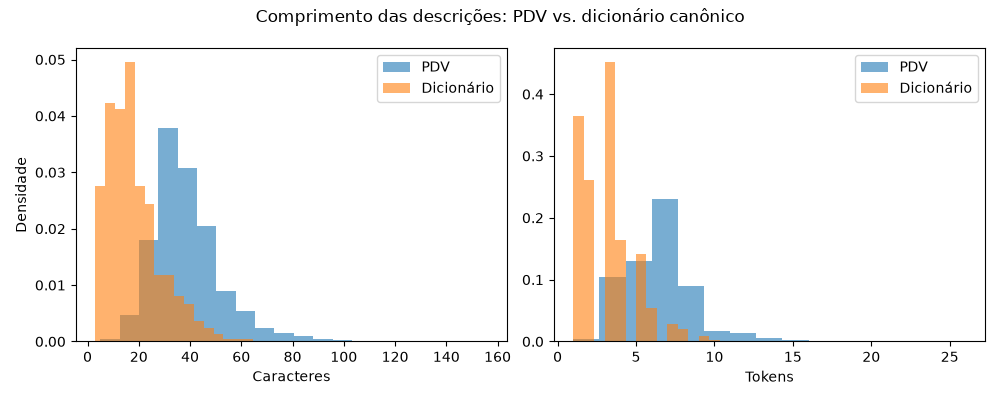
\includegraphics[width=\textwidth]{fig_comprimento_descricoes.png}
\vspace{2mm}
\fonte{Elaborado pelo autor a partir de dados do projeto ALTA}
\end{figure}


Quanto ao ruído, 90,3\% das descrições trazem a quantidade colada à unidade de medida (por exemplo, \texttt{500G}), 74,2\% não contêm nenhum caractere acentuado, 24,0\% estão inteiramente em caixa alta e 3,4\% exibem marca explícita de abreviação ou truncamento --- este último, um piso, já que abreviações sem marca gráfica não são detectadas. Cada unidade de medida aparece em várias grafias; grama, por exemplo, em cinco (Tabela~\ref{tab:formas-unidade}). Além disso, 376 grupos de produtos aparecem com os mesmos tokens em ordens diferentes entre redes. A Tabela~\ref{tab:exemplos-ruido} reúne exemplos reais de cada tipo; nos pares de unidade, as duas descrições são de produtos diferentes e ilustram apenas a variação de grafia da mesma unidade. A unidade estruturada (campos de valor e unidade normalizados) está ausente em 5,9\% dos registros e quase nunca é recuperável a partir do texto da descrição, o que limita a supervisão distante e, na fatia produto--produto, a comparação de tamanho entre itens vendidos a peso ou por unidade.

% Gerado automaticamente por scripts/02_analise_exploratoria.py — não editar à mão.
\begin{table}[htbp]
\centering
\caption{Grafias observadas por unidade de medida}
\label{tab:formas-unidade}
\small
\begin{tabular}{llr}
\toprule
Unidade & Grafia & Contagem \\
\midrule
grama & g & 13164 \\
mililitro & ml & 5239 \\
grama & G & 3155 \\
mililitro & ML & 1899 \\
quilograma & kg & 1149 \\
grama & GR & 1091 \\
litro & l & 910 \\
litro & L & 581 \\
quilograma & Kg & 222 \\
quilograma & KG & 165 \\
unidade & und & 103 \\
litro & LT & 96 \\
grama & gr & 31 \\
mililitro & Ml & 26 \\
litro & lt & 24 \\
unidade & UN & 19 \\
unidade & un & 9 \\
unidade & Und & 4 \\
unidade & UND & 4 \\
mililitro & mL & 4 \\
grama & Gr & 1 \\
\bottomrule
\end{tabular}
\vspace{2mm}
\fonte{Elaborado pelo autor a partir de dados do projeto ALTA}
\end{table}


% Gerado automaticamente por scripts/02_analise_exploratoria.py — não editar à mão.
\begin{table}[htbp]
\centering
\caption{Exemplos reais por tipo de ruído de PDV}
\label{tab:exemplos-ruido}
\small
\resizebox{\textwidth}{!}{%
\begin{tabular}{lll}
\toprule
Tipo de ruído & Descrição A & Descrição B \\
\midrule
abreviação & Abobrinha 1kg (aprox. 3und.) &  \\
abreviação & CAFE SOLUVEL S.BRAZ EF.100GR VIDRO &  \\
abreviação & GELEIA TRADL AMORA C/PEDACOS CASA MADEIRA 240G &  \\
tipografia & DOCE POTE CAJU KELLY CREMER CRISTAL 300G &  \\
tipografia & Biscoito Milka Choco Creme Recheado De Chocolate Ao Leite 260g  &  \\
tipografia & File De Coxa Frango Iqf Swift 1 Kg &  \\
unidade & MOLHO TOMATE TRADICIONAL HEMMER SC 300G & KETCHUP HELLMANNS TRAD SQUEEZE 390GR SUPREME \\
unidade & VINHO PORT GATAO RS 750ML & Sorvete Tapioca La Basque 490Ml \\
unidade & FARINHA PANKO ROMARIZ 1KG & Bacalhau do Porto Morhua Resfriado 2,5Kg \\
inversão & Suco de Uva Campo Largo Integral 1,35L & Suco De Uva Integral Campo Largo 1,35l \\
inversão & Água Mineral Crystal Sem Gás 1,5l & Água Mineral sem Gás Crystal 1,5L \\
inversão & Suco Frut Frutas Cítricas Del Valle 1,5L & Suco Del Valle Frut Frutas Citricas 1,5l \\
\bottomrule
\end{tabular}%
}
\vspace{2mm}
\fonte{Elaborado pelo autor a partir de dados do projeto ALTA}
\end{table}


O vocabulário evidencia a especificidade do domínio (Tabela~\ref{tab:vocabulario}): dos 10.031 tipos de token, após normalização, 37\% ocorrem uma única vez e 60\% aparecem em uma única rede; a similaridade de Jaccard entre os vocabulários das redes varia de 0,08 a 0,37 (Figura~\ref{fig:jaccard-lojas}); e 92\% dos tipos de token da base não ocorrem no vocabulário do dicionário canônico.

% Gerado automaticamente por scripts/02_analise_exploratoria.py — não editar à mão.
\begin{table}[htbp]
\centering
\caption{Vocabulário e dispersão lexical entre lojas}
\label{tab:vocabulario}
\small
\begin{tabular}{lr}
\toprule
Métrica & Valor \\
\midrule
Tipos (bruto, sensível a caixa/acento) & 13846 \\
Tipos (normalizado) & 10031 \\
Hapax legomena (frequência 1) & 3612 \\
Dis legomena (frequência 2) & 1412 \\
Tokens exclusivos de uma loja & 5976 \\
— idem, com frequência $\geq$ 2 & 2364 \\
Vocabulário do dicionário canônico & 1095 \\
— presente na base bruta & 799 \\
Cobertura do dicionário na base (\%) & 73.0 \\
Tokens brutos fora do dicionário (OOV, \%) & 92.0 \\
\bottomrule
\end{tabular}
\vspace{2mm}
\fonte{Elaborado pelo autor a partir de dados do projeto ALTA}
\end{table}


% Gerado automaticamente por scripts/02_analise_exploratoria.py — não editar à mão.
\begin{figure}[htbp]
\centering
\caption{Similaridade de Jaccard do vocabulário entre lojas}
\label{fig:jaccard-lojas}
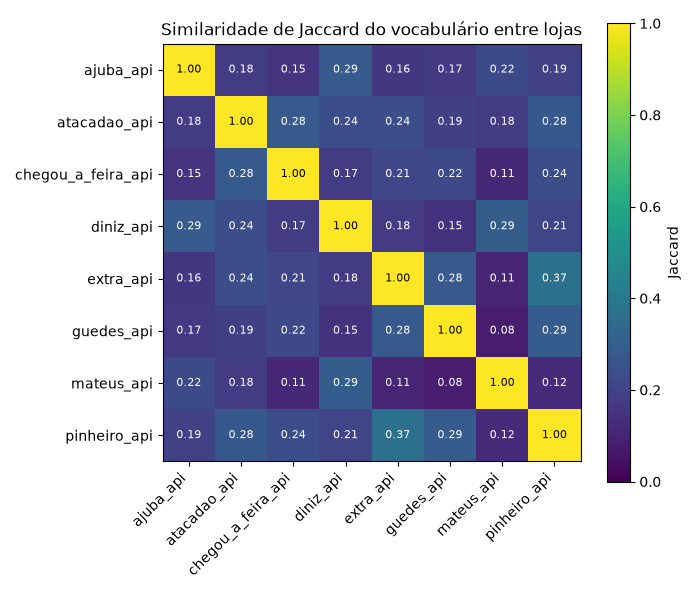
\includegraphics[width=0.8\textwidth]{fig_jaccard_lojas.png}
\vspace{2mm}
\fonte{Elaborado pelo autor a partir de dados do projeto ALTA}
\end{figure}


A distribuição de produtos por categoria não é reportada: a coluna candidata do dicionário (\texttt{cod\_padrao}) tem significado não confirmado com o time do ALTA e concentra 82,7\% das entradas em um único valor, e optou-se por não utilizá-la como campo de categoria. A proporção entre pares de match e não-match será conhecida somente após a construção do conjunto rotulado e reportada junto às métricas do conjunto de dados.

% ============================================================
% 5. CRONOGRAMA DE EXECUÇÃO
% ============================================================
\section{Cronograma de Execução}

O trabalho é planejado para execução individual ao longo de dezesseis semanas, com dedicação parcial. Os marcos possuem critério de conclusão verificável. Dada a criticidade da construção do ground truth, adota-se a regra de que eventuais atrasos serão absorvidos pela etapa de ablação (Semana 13), nunca pela etapa de anotação ou pela redação.

\textbf{Redação incremental.} Para mitigar o risco de concentrar a redação do TCC em uma única semana final, a Introdução, a Revisão de Literatura e a Metodologia são redigidas em paralelo à execução técnica, ao longo das Semanas 1 a 9 --- seções que não dependem de resultados experimentais. Um checkpoint de escrita ao final da Semana 8 exige pelo menos 60\% do texto do TCC redigido (todas as seções exceto Resultados e Discussão). Isso libera a Semana 15 exclusivamente para a redação de Resultados, Discussão e Conclusão, e reserva espaço explícito para revisão do orientador antes da entrega final.

\begin{longtable}{p{1.8cm} p{6.5cm} p{6.2cm}}
\caption{Cronograma por semanas, fases e marcos}
\label{tab:cronograma} \\
\toprule
\textbf{Semanas} & \textbf{Fase / Atividade} & \textbf{Critério de conclusão} \\
\midrule
\endfirsthead

\multicolumn{3}{c}{\tablename\ \thetable\ -- continuação} \\
\toprule
\textbf{Semanas} & \textbf{Fase / Atividade} & \textbf{Critério de conclusão} \\
\midrule
\endhead

\bottomrule
\multicolumn{3}{r}{\textit{continua}} \\
\endfoot

\bottomrule
\endlastfoot

1 & Análise exploratória da base; definição do protocolo de anotação & Estatísticas descritivas documentadas; protocolo escrito \\
2 & Geração de candidatos (blocagem produto--dicionário e produto--produto; supervisão distante) e configuração do treino & Pipeline de \textit{bootstrapping} funcional \\
3--5 & Anotação manual do conjunto de teste padrão-ouro (fatias produto--produto e produto--dicionário) e teste-reteste \newline \textit{Redação: Introdução} & Conjunto de teste anotado; Kappa intra-anotador calculado \\
6 & Partição anti-vazamento (nenhum produto em mais de uma partição) e aumentação sintética do treino \newline \textit{Redação: Revisão de Literatura} & Partições versionadas; conjunto de treino gerado \\
7--8 & Implementação e avaliação dos baselines clássicos \newline \textit{Redação: Metodologia} & Tabela de baselines fechada; harness reproduzível; checkpoint: $\geq$60\% do TCC redigido \\
9 & Configuração do SLM (dois adaptadores LoRA bf16), formatação dos pares, seeds e configs & Pipeline de treino executa de ponta a ponta \\
10--11 & Fine-tuning, ajuste de hiperparâmetros e mineração de negativos difíceis & Modelo treinado; curvas de treino registradas \\
12 & Avaliação do modelo vs. baselines, por fatia; teste de significância estatística & Tabela comparativa; hipótese central testada \\
13 & Ablação enxuta (aumentação; negativos difíceis); análise de pipeline progressivo & Dois estudos de ablação documentados; economia computacional do pipeline progressivo quantificada \\
14 & Análise de erro qualitativa por tipo de ruído & Taxonomia de erros e exemplos \\
15 & Redação de Resultados, Discussão e Conclusão; entrega de rascunho completo ao orientador no início da semana & Rascunho completo entregue; retorno do orientador obtido até o final da semana \\
16 & Incorporação do feedback do orientador, revisão final, formatação ABNT e preparação da defesa & TCC entregue; slides prontos \\

\end{longtable}
\vspace{-4mm}
\fonte{Elaborado pelo autor}


A redação do artigo de conferência será conduzida a partir do TCC, posteriormente à Semana 16, com folga em relação à entrega institucional.

% ============================================================
% 6. JUSTIFICATIVA E CONTRIBUIÇÃO CIENTÍFICA
% ============================================================
\section{Justificativa e Contribuição Científica}

\subsection{Relevância aplicada}

O problema de Entity Matching em bases de preços de varejo possui impacto direto na qualidade das análises do projeto ALTA/CNPq. Sem a resolução de entidades, registros do mesmo produto em lojas diferentes permanecem incomparáveis, inviabilizando estudos de cesta básica, análise de competitividade regional e monitoramento inflacionário. A solução desenvolvida contribui diretamente para a infraestrutura analítica do projeto.

\subsection{Lacuna científica}

Conforme detalhado na revisão de literatura, a pesquisa em EM concentra-se em dados estruturados em inglês, com benchmarks consolidados. O matching de produtos em português brasileiro, com o perfil de ruído específico de sistemas de PDV de varejo regional, constitui cenário pouco explorado. O fine-tuning de um SLM para este domínio representa uma contribuição metodológica original, especialmente por operar em regime de baixo recurso, a partir de ausência total de rótulos.

\subsection{Hipótese central}
\label{sec:hipotese-central}

A hipótese central deste trabalho é que um SLM com fine-tuning supervisionado no domínio de produtos de supermercado supera tanto os métodos tradicionais de similaridade de strings quanto o mesmo modelo sem especialização (zero-shot) na decisão de se duas descrições de lojas distintas correspondem ao mesmo produto, mesmo com um conjunto de treinamento de escala moderada. Como hipótese secundária, o mesmo vale para o mapeamento de produtos ao dicionário canônico, avaliado com adaptador próprio e reportado separadamente. Dado o tamanho dos conjuntos de teste (Seção~\ref{sec:construcao-dataset}), a significância estatística é avaliada por teste pareado adequado à comparação de classificadores sobre o mesmo conjunto (por exemplo, teste de McNemar), reportando-se também o tamanho do efeito e os intervalos de confiança independentemente do resultado do teste de hipótese --- uma vez que, com esse N, diferenças de pequena magnitude podem não atingir significância estatística sem que isso invalide a direção do efeito observado.

\subsection{Alinhamento com o horizonte de pesquisa}

O trabalho é concebido para produzir três entregas simultâneas: o TCC como entrega institucional na UFPB; um artigo científico submetível a conferência nacional; e uma base metodológica sólida para possível continuidade em programa de pós-graduação. O desenvolvimento ocorre com infraestrutura da Dharma-AI, startup especializada em fine-tuning de SLMs para domínios específicos, o que assegura recursos computacionais adequados e conhecimento técnico especializado. O uso desses recursos é conduzido com conhecimento interno da empresa, da qual o autor é colaborador; [a confirmar formalmente, por escrito, com a liderança da Dharma-AI: autorização para uso de sua infraestrutura e ferramenta de geração de dados no âmbito deste TCC.] [a levantar com o orientador, antes da defesa: avaliação conjunta do potencial de proteção por patente ou registro sobre a solução desenvolvida (modelo fine-tuned, pipeline ou artefatos gerados); a conversa ainda não ocorreu, e a decisão sobre o que abrir e quando depende de seu resultado.]

% ============================================================
% 7. TRABALHOS FUTUROS
% ============================================================
\section{Trabalhos Futuros}

Delimitações de escopo adotadas neste trabalho, motivadas pelo horizonte temporal de dezesseis semanas em execução individual, definem direções naturais de continuidade:

\begin{itemize}
    \item Arquiteturas Bi-Encoder e híbrida (recuperação neural seguida de reranqueamento) --- direções reconhecidamente promissoras (Seção~\ref{sec:objetivos-especificos}), situadas fora do escopo deste trabalho em favor da formulação de Cross-Encoder único;
    \item Blocagem com representações de subpalavra (n-gramas de caracteres) ou aprendidas, para recuperar os pares sem sobreposição lexical que a blocagem clássica perde (Seção~\ref{sec:blocagem});
    \item Transferência de domínio a partir de benchmarks de EM em inglês, seguida de fine-tuning no domínio de produtos em português brasileiro;
    \item Publicação do conjunto de teste anotado como benchmark aberto de EM de produtos em português brasileiro, mediante autorização dos coordenadores do projeto ALTA/CNPq.
\end{itemize}

% \begin{dica}
% \noindent\textbf{Dica ao autor — Como escrever Resultados e Discussão:}
%
% Esta é a seção mais importante. Siga o padrão \textbf{OII} para cada resultado:
% \begin{enumerate}
%     \item \textbf{Observação:} O que os dados mostram? (fato objetivo)
%     \item \textbf{Interpretação:} O que isso significa? (sua análise)
%     \item \textbf{Implicação:} Como se relaciona com a literatura? (conexão)
% \end{enumerate}
% \textbf{Exemplo:} ``O LightGBM obteve AUC-ROC de 0,877, superando a Regressão Logística (0,823). [Observação] O desempenho superior pode ser atribuído à capacidade de capturar interações não-lineares. [Interpretação] Este resultado corrobora Fernandes (2023), que obteve AUC de 0,89 com dados reais. [Implicação]''
%
% \textbf{Erros comuns:} (1)~Apenas descrever tabelas sem interpretar: ``A Tabela~3 mostra os resultados.'' — e daí? (2)~Não comparar com a literatura. (3)~Ignorar resultados negativos --- se algo não funcionou, explique por quê. Toda figura e tabela \textbf{deve ser mencionada e interpretada no texto}.
% \end{dica}
%
% \begin{dica}
% \noindent\textbf{Dica ao autor — Como escrever as Considerações Finais:}
%
% A conclusão \textbf{não} é um resumo do trabalho. É uma avaliação de fechamento. Estruture assim:
% \begin{enumerate}
%     \item \textbf{Retomada dos objetivos:} Cada objetivo específico foi alcançado? Avalie honestamente.
%     \item \textbf{Contribuições:} O que o trabalho acrescenta ao campo? (1 parágrafo)
%     \item \textbf{Limitações:} O que não foi possível fazer e por quê? Reconhecer limitações demonstra \textbf{maturidade intelectual} --- os avaliadores valorizam isso.
%     \item \textbf{Trabalhos futuros:} Sugestões concretas e viáveis para pesquisas subsequentes.
% \end{enumerate}
% \textbf{Regras de ouro:}
% \begin{itemize}
%     \item Não introduza referências novas nem dados que não foram discutidos.
%     \item Não comece com ``Em suma'' ou ``Portanto'' --- comece com conteúdo substantivo.
%     \item Seja específico nos trabalhos futuros: ``testar SMOTE para balanceamento'' é melhor que ``explorar outras técnicas''.
% \end{itemize}
% \end{dica}
% Nota: as duas dicas acima (Resultados/Discussão e Considerações Finais) são preservadas do
% template original; este documento é a PROPOSTA (sem essas seções ainda) — aplicam-se na
% versão final do TCC (spec 005), quando as seções Resultados, Discussão e Conclusão existirem.

% ============================================================
% 8. REFERÊNCIAS
% ============================================================
\bibliographystyle{abntex2-alf}
\bibliography{referencias}

\end{document}
